\documentclass[a4paper]{jpconf}
\usepackage{graphicx}
\usepackage{amsmath,bm,dsfont,amssymb,amsfonts}

%\usepackage{autonum}
\renewcommand\[{\begin{equation}}
\renewcommand\]{\end{equation}}

\newcommand{\ssigma}{{\bm \sigma}}

\newcommand{\be}{\begin{equation}}
\newcommand{\ee}{\end{equation}}

\newcommand{\A}{{\cal A}}
\newcommand{\B}{{\cal B}}


%\usepackage[backend=biber]{biblatex}
%\bibliography{biblio}
%%\bibliographystyle{iopart-num}

\begin{document}
\title{A variational lower bound on the ground state of a many-body system and the squaring parametrization of density matrices}

\author{F. Uskov$^1$,  O. Lychkovskiy$^{1,2}$}

\address{$^1$ Skolkovo Institute of Science and Technology,	Nobel street 3, Moscow  121205, Russia}
\address{$^2$ Steklov Mathematical Institute of Russian Academy of Sciences,	Gubkina str., 8, Moscow 119991, Russia}

\ead{fel1992@mail.ru}

\begin{abstract}
A variational {\it upper} bound on the ground state energy $E_{\rm gs}$ of a quantum system, $E_{\rm gs} \leqslant \langle \Psi|H| \Psi \rangle$, is well-known (here $H$ is the Hamiltonian of the system and $\Psi$ is an arbitrary wave function). Much less known are variational {\it lower} bounds on the ground state. We consider one such bound which is valid for a many-body translation-invariant lattice system. Such a lattice can be divided into clusters which are identical up to translations. The Hamiltonian of such a system can be written as $H=\sum_{i=1}^M H_i$, where a term $H_i$ is supported on the $i$'th cluster. The bound reads $E_{\rm gs}\geqslant M \inf\limits_{\rho_{cl} \in {\mathbb S_{cl}^G}} \tr_{cl}\rho_{cl} \, H_{cl} $, where ${\mathbb S_{cl}^G}$ is some wisely chosen set of reduced density matrices of a single cluster. The implementation of this latter variational principle can be hampered by the difficulty of parameterizing the set  $\mathbb M$, which is a necessary prerequisite for a variational procedure. The root cause of this difficulty is the nonlinear positivity constraint $\rho>0$ which is to be satisfied by a density matrix. The squaring parametrization of the density matrix, $\rho=\tau^2/\tr\tau^2$, where $\tau$ is an arbitrary (not necessarily positive) Hermitian operator, accounts for positivity automatically. We discuss how the squaring parametrization can be utilized to find variational lower bounds on ground states of translation-invariant many-body systems. As an example, we consider a one-dimensional Heisenberg antiferromagnet.
\end{abstract}

\section{Introduction}
The ground state of a many-particle system is one of the central objects studied in condensed matter physics.
The ground state energy as a rule cannot be calculated exactly.
In strongly correlated systems, it is also difficult to apply the perturbation theory. A common way to asses the ground state energy is via variational methods. An upper bound on the ground state energy, $E_{\rm gs} \leqslant \langle \Psi|H| \Psi \rangle$, is well-known.
It is often desirable to supplement the latter with a {\it lower} bound.
Methods for obtaining lower bounds on ground state energies of many-body systems exist \cite{Anderson,NishimoriOzeki,MattisPan,Mazziotti,Baumgratz}, but they are much less developed than standard variational methods.
In this paper we suggest  one such method applicable to translation-invariant lattice systems with local interactions. The method is applied to a simple system, and its merits and prospects are discussed.

\section{Lower bound on the ground state energy of a translation-invariant lattice system}

\subsection{Our lower bound}

\begin{figure}[t]
	\begin{minipage}{7pc}
		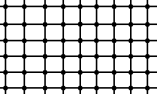
\includegraphics[width=7pc]{sqlattice.png}
	\end{minipage}\hspace{2pc}%
	\begin{minipage}{7pc}
		\caption{\label{label} Square lattice.}
	\end{minipage}\hspace{2pc}%
	\begin{minipage}{7pc}
		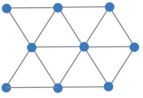
\includegraphics[width=7pc]{triangle-lattice.png}
	\end{minipage}\hspace{2pc}%
	\begin{minipage}{7pc}
		\caption{\label{label} Triangular  lattice.}
	\end{minipage}
\end{figure}
We consider a system of spins on a lattice with $N$ sites. The lattice is invariant with respect to the group of translation and, for two- and three-dimensional lattices, rotations. For example, this can be a linear chain in one dimension and a square or a triangular lattice in two dimensions, see Figures 1,2.  Due to the symmetry, a lattice can be divided into identical clusters. The Hamiltonian of the system is defined on the lattice and is invariant under a group $G$ which contains the symmetries of the lattice and, in general, some other symmetries,
\be
U\,H\,U^\dagger =H~~~~~\forall ~~U\in G.
\ee 
The Hamiltonian  can be written as
\be\label{H}
H=\sum_{i=1}^M H_i,
\ee
where $H_i$ is the local Hamiltonian of the $i$'th cluster, and the total number of clusters is $M$. In what follows we will use a special notation $H_cl\equiv H_1$ for the first cluster. Local terms $H_i$ can be transformed one to another by group actions, i.e.
\be\label{Hi}
H_i=U\,H_j\,U^\dagger~~~~{\rm for~ some}~~~U\in G. 
\ee

Now let us derive our variational lower bound. First we note that the ground state energy of the system is given variationally by 
\[
E_{gs} = 
\inf\limits_{ \rho \in {\mathbb S}^G} \mathop{\rm{tr}} H \rho,
\]
where  ${\mathbb S}^G$ is a set of density matrices $\rho$  invariant under the group $G$ \cite{Shpagina}. Further, using eqs. \eqref{H} and \eqref{Hi}, we get 
\[\label{Egs 2}
E_{gs} =
M \inf\limits_{ \rho \in {\mathbb S}^G} \tr_{cl} \left( H_{cl} \tr_{\overline{cl}}\rho\right),
\]
where $\tr_{cl}$ and $\tr_{\overline{cl}}$ are partial traces over the cluster and its complement, respectively. Note that while $\rho_{cl}\equiv\tr_{\overline{cl}}\rho$ is just the reduced density matrix of the cluster, variation in eq. \eqref{Egs 2} is not performed over the set of {\it all} $\rho_{cl}$. Instead, the minimization is effectively performed over those $\rho_{cl}$ which can be obtained from $\rho \in {\mathbb S}^G$. The set of $\rho_{cl}$ satisfying the latter condition is unknown. However, we can lower bound $E_{gs}$ by performing minimization over a larger set ${\mathbb S}_{cl}^G$ of the reduced density matrices of the cluster symmetric under the group $G$. This way we obtain our variational lower bound
\[\label{our bound}
E_{gs} \geq 
M \inf\limits_{ \rho_{cl} \in {\mathbb S}_{cl}^G} \tr_{cl}  H_{cl} \rho_{cl}.
\]
This bound is the main general result of the present paper. It should be stressed that $H_{cl}$ is {\it not} invariant under  the group $G$, in contrast to $\rho_{cl} \in {\mathbb S}_{cl}^G$.


We further observe that this bound can be enhanced by requiring that $\rho_{cl}$ satisfies local sum rules which follow from the anti-Hermitian Stationary Schr\"odinger equation \cite{Shpagina}. 

\subsection{Density matrix parametrization}
In order to be able to perform minimization in eq. \eqref{our bound} one needs to parameterize the set ${\mathbb S}_{cl}^G$ of density matrices. Remind that any density matrix must satisfy three conditions,
\[{\rho ^ \dagger } = \rho ;\qquad \mathop{\rm{tr}}\rho  = 1;\qquad  \rho  > 0. \label{conditions on rho}\]
The positivity condition is nonlinear and thus the most problematic. A squaring parametrization has been developed in \cite{SqParam} which automatically accounts for the positivity as well as other two conditions. In addition, it is well suted for many-body systems and for accounting for symmetries. Its main idea is that if we take an arbitrary hermitian matrix $\tau$, and square it and normalize it, we get a valid density matrix:
\[\rho  = \frac{{{\tau ^2}}}{{\mathop{\rm{tr}}{\tau ^2}}},~~~~~~{\rm where}~~~~~ {\tau ^ + } = \tau. \label{tau}\]
We will us the squaring parametrization of density matrices to practically apply the bound \eqref{our bound}.



\subsection{Comparison to the Anderson bound}

Let us remind the Anderson bound, which is arguably the first and the most widely used lower bound on $E_{gs}$ \cite{Anderson}. It is based on a simple fact that infimum of a sum is greater than the sum of infimums. This leads to the bound
\be
E_{gs} \geq
M \inf\limits_{ \rho_{cl} } \, \tr_{cl}  H_{cl} \rho_{cl}.
\ee
The infimum here is taken over all density matrices $\rho_{cl}$ of a cluster. For this reason, the Anderson bound is weaker than our bound \eqref{our bound}.

\section{Application to a system of spins $1/2$ with Heisenberg interactions}

\subsection{Spin systems with Heisenberg interactions}

In the present section we show how the bound \eqref{our bound} can be applied to  a system of $N$ spins with the Heisenberg interaction. The Hamiltonian of this system reads
%
\begin{equation}\label{H Heisenberg}
	H = \sum_{<i,j>} \left( {{{\bm \ssigma}_i}{{\bm \ssigma}_j}} \right) ,
\end{equation}
where  the sum is taken over all neighbouring sites on the lattice, ${\bm \ssigma}_i$ is the vector consisting of three Pauli matrices of the $i$'th spin and $\left( {{{\bm \ssigma}_i}{{\bm \ssigma}_j}} \right)$ is the corresponding scalar product of sigma-matrices. This Hamiltonian is invariant with respect to a global $SU(2)$ symmetry, in other words, to the simultaneous rotations of all spins. It is also invariant under inversion of time and respects the spatial symmetries of the lattice. 

As is discussed in details in \cite{SqParam,Shpagina}, a density matrix $\rho$ and matrix $\tau$ from eq. \eqref{tau} can be expressed in terms of scalar products of sigma matrices,
\[
\def\arraystretch{1.8}
\begin{array}{l}
\rho  = 2^{-N} \sum_\A a_\A A_\A;\qquad \qquad \tau  = \sum_\A b_\A A_\A
\\
\{ A_\A \}  = \{ 1,  \;\;({\bf \ssigma}_j{\bf\ssigma}_k), \;\;
({\bf \ssigma}_j{\bf\ssigma}_k)({\bf \ssigma}_l{\bf\ssigma}_m)\;\;,\;\;...\},~~i,k,l,m,...=1,2,...N.
\end{array}\]
Here $b_i$ are arbitrary real numbers while $a_i$ are some functions of $b_i$ determined by eq. \eqref{tau}.

Let us make several remarks concerning the algebra of $A_\A$. First, we list useful relations,
\[\begin{array}{l}
{({{\ssigma}_1}{{\ssigma}_2})^2}\qquad \quad {\mkern 1mu} {\mkern 1mu}  = \;\;{\mkern 1mu} 3 - 2({{\ssigma}_1}{{\ssigma}_2})\\
({{\ssigma}_1}{{\ssigma}_2})({{\ssigma}_2}{{\ssigma}_3})\;\;\;\; = \;\;\;({{\ssigma}_1}{{\ssigma}_3}) - i({{\ssigma}_1}{{\ssigma}_2}{{\ssigma}_3})\\
({{\ssigma}_1}{{\ssigma}_2})({{\ssigma}_1}{{\ssigma}_2}{{\ssigma}_3}) =  - ({{\ssigma}_1}{{\ssigma}_2}{{\ssigma}_3}) - 2i({{\ssigma}_1}{{\ssigma}_3}) + 2i({{\ssigma}_2}{{\ssigma}_3})\\
({{\ssigma}_1}{{\ssigma}_2}{{\ssigma}_3})({{\ssigma}_1}{{\ssigma}_2}) =  - ({{\ssigma}_1}{{\ssigma}_2}{{\ssigma}_3}) + 2i({{\ssigma}_1}{{\ssigma}_3}) - 2i({{\ssigma}_2}{{\ssigma}_3})\\
({{\ssigma}_1}{{\ssigma}_2})({{\ssigma}_2}{{\ssigma}_3}{{\ssigma}_4}) = ({{\ssigma}_1}{{\ssigma}_3}{{\ssigma}_4}) - i({{\ssigma}_1}{{\ssigma}_3})({{\ssigma}_2}{{\ssigma}_4}) + i({{\ssigma}_1}{{\ssigma}_4})({{\ssigma}_2}{{\ssigma}_3})\\
({{\ssigma}_2}{{\ssigma}_3}{{\ssigma}_4})({{\ssigma}_1}{{\ssigma}_2}) = ({{\ssigma}_1}{{\ssigma}_3}{{\ssigma}_4}) + i({{\ssigma}_1}{{\ssigma}_3})({{\ssigma}_2}{{\ssigma}_4}) - i({{\ssigma}_1}{{\ssigma}_4})({{\ssigma}_2}{{\ssigma}_3})\\
{({{\ssigma}_1}{{\ssigma}_2}{{\ssigma}_3})^2}{\mkern 1mu} {\mkern 1mu} {\mkern 1mu} \qquad {\mkern 1mu}  = 6 - 2({{\ssigma}_1}{{\ssigma}_2}) - 2({{\ssigma}_1}{{\ssigma}_3}) - 2({{\ssigma}_2}{{\ssigma}_3})\\
({{\ssigma}_1}{{\ssigma}_2}{{\ssigma}_3})({{\ssigma}_1}{{\ssigma}_2}{{\ssigma}_4}) =  - ({{\ssigma}_1}{{\ssigma}_3})({{\ssigma}_2}{{\ssigma}_4}) - ({{\ssigma}_1}{{\ssigma}_4})({{\ssigma}_2}{{\ssigma}_3}) + 2({{\ssigma}_3}{{\ssigma}_4}) + i({{\ssigma}_1}{{\ssigma}_3}{{\ssigma}_4}) + i({{\ssigma}_2}{{\ssigma}_3}{{\ssigma}_4})\\
({{\ssigma}_1}{{\ssigma}_2}{{\ssigma}_3})({{\ssigma}_1}{{\ssigma}_4}{{\ssigma}_5}) =  + ({{\ssigma}_2}{{\ssigma}_4})({{\ssigma}_3}{{\ssigma}_5}) - ({{\ssigma}_2}{{\ssigma}_5})({{\ssigma}_3}{{\ssigma}_4}) - i({{\ssigma}_1}{{\ssigma}_2})({{\ssigma}_3}{{\ssigma}_4}{{\ssigma}_5}) + i({{\ssigma}_1}{{\ssigma}_3})({{\ssigma}_2}{{\ssigma}_4}{{\ssigma}_5}),
\end{array}\]
where $({{\ssigma}_1}{{\ssigma}_2}{{\ssigma}_3})$ is the mixed product of sigma matrices. Further, a product of two mixed products can always be represented through scalar products:
\[{\rm{(}}{{\ssigma}_1}{{\ssigma}_2}{{\ssigma}_3}{\rm{)(}}{{\ssigma}_4}{{\ssigma}_5}{{\ssigma}_6}{\rm{) = }}\det \left( {\begin{array}{*{20}{c}}
	{{\rm{(}}{{\ssigma}_1}{{\ssigma}_4}{\rm{)}}}&{{\rm{(}}{{\ssigma}_2}{{\ssigma}_4}{\rm{)}}}&{{\rm{(}}{{\ssigma}_3}{{\ssigma}_4}{\rm{)}}}\\
	{{\rm{(}}{{\ssigma}_1}{{\ssigma}_5}{\rm{)}}}&{{\rm{(}}{{\ssigma}_2}{{\ssigma}_5}{\rm{)}}}&{{\rm{(}}{{\ssigma}_3}{{\ssigma}_5}{\rm{)}}}\\
	{{\rm{(}}{{\ssigma}_1}{{\ssigma}_6}{\rm{)}}}&{{\rm{(}}{{\ssigma}_2}{{\ssigma}_6}{\rm{)}}}&{{\rm{(}}{{\ssigma}_3}{{\ssigma}_6}{\rm{)}}}
	\end{array}} \right)
\label{mixeddet}
.\]

One can introduce scalar product on the space of operators according to 
\[(A,B) \equiv \mathop{\rm{tr}}(A^+ B) = \mathop{\rm{tr}}(AB);\qquad {A^ + } = A\]
(not to be confused with the scalar product of sigma matrices).
If supports of $A$ and $B$ on a lattice do not coincide, then $(A,B) = 0$.
If $A$ and $B$ have the same support, then $\left( {A,B} \right) = {2^N}{3^C}$,
where $N$ - is number of spins and $C$ - is the number of cycles  arising when the bonds contained in $A$ are superimposed on the bonds contained in $B$ ({\it cf.} ref. \cite{BeachSandvik}). In particular,
\[{\rm{tr}}(\;({{\ssigma}_i}{{\ssigma}_j})({{\ssigma}_j}{{\ssigma}_k})...({{\ssigma}_l}{{\ssigma}_m})({{\ssigma}_m}{{\ssigma}_i})\;) = 3 \cdot {2^N}\]
(one cycle) and 
\[
{\rm{tr}}(\;({{\ssigma}_i}{{\ssigma}_j}{{\ssigma}_k})({{\ssigma}_i}{{\ssigma}_j}{{\ssigma}_n})\;({{\ssigma}_k}{{\ssigma}_l})...({{\ssigma}_m}{{\ssigma}_n})\;) =
{\rm{tr}}(\;({{\ssigma}_i}{{\ssigma}_j}{{\ssigma}_k})({{\ssigma}_i}{{\ssigma}_j}{{\ssigma}_k})\;) = 6 \cdot {2^N}.
\]

\subsection{Properties  of the set $\{A_\A\}$}
Let us consider a set  ${B_\B}$ of the following form:
$$
\{ B_\B \}  = \{ ({\bf \ssigma}_p{\bf\ssigma}_r{\bf\ssigma}_s),\;\;
({\bf \ssigma}_p{\bf\ssigma}_r{\bf\ssigma}_s)({\bf \ssigma}_j{\bf\ssigma}_k), \;\;
({\bf \ssigma}_p{\bf\ssigma}_r{\bf\ssigma}_s)({\bf \ssigma}_j{\bf\ssigma}_k)({\bf \ssigma}_l{\bf\ssigma}_m)\;\;,\;\;...\}
$$

Bases $\{A_\A\}$ and $\{A_\A,B_\B\}$ are not orthogonal, for example
\[\begin{array}{l}
\qquad \qquad \quad {\rm{A = (}}{{\ssigma}_1}{{\ssigma}_2}{\rm{)(}}{{\ssigma}_3}{{\ssigma}_4}{\rm{)}}\\
\qquad \qquad \quad {\rm{B = (}}{{\ssigma}_1}{{\ssigma}_3}{\rm{)(}}{{\ssigma}_2}{{\ssigma}_4}{\rm{)}}\\
\qquad \qquad \quad {\rm{C = (}}{{\ssigma}_1}{{\ssigma}_4}{\rm{)(}}{{\ssigma}_2}{{\ssigma}_3}{\rm{)}}\\
g = \left( {\begin{array}{*{20}{c}}
	{(AA)}&{(AB)}&{(AC)}\\
	{(BA)}&{(BB)}&{(BC)}\\
	{(CA)}&{(CB)}&{(CC)}
	\end{array}} \right) = \left( {\begin{array}{*{20}{c}}
	9&3&3\\
	3&9&3\\
	3&3&9
	\end{array}} \right) > 0
\end{array}\]

Also they are over-complete. However, we suggest that  all linear dependencies within the basis can be described by 
\[{\rm{ + (}}{{\ssigma}_1}{{\ssigma}_2}{\rm{)(}}{{\ssigma}_3}{{\ssigma}_4}{{\ssigma}_5}{\rm{) - (}}{{\ssigma}_1}{{\ssigma}_3}{\rm{)(}}{{\ssigma}_2}{{\ssigma}_4}{{\ssigma}_5}{\rm{)}} + {\rm{(}}{{\ssigma}_1}{{\ssigma}_4}{\rm{)(}}{{\ssigma}_2}{{\ssigma}_3}{{\ssigma}_5}{\rm{) - (}}{{\ssigma}_1}{{\ssigma}_5}{\rm{)(}}{{\ssigma}_2}{{\ssigma}_3}{{\ssigma}_4}{\rm{)}} = 0
\label{basisdep}
\]
for elements with an odd number of spins, and by
\[\det \left( {\begin{array}{*{20}{c}}
	{{\rm{(}}{{\ssigma}_1}{{\ssigma}_5}{\rm{)}}}&{{\rm{(}}{{\ssigma}_2}{{\ssigma}_5}{\rm{)}}}&{{\rm{(}}{{\ssigma}_3}{{\ssigma}_5}{\rm{)}}}&{{\rm{(}}{{\ssigma}_4}{{\ssigma}_5}{\rm{)}}}\\
	{{\rm{(}}{{\ssigma}_1}{{\ssigma}_6}{\rm{)}}}&{{\rm{(}}{{\ssigma}_2}{{\ssigma}_6}{\rm{)}}}&{{\rm{(}}{{\ssigma}_3}{{\ssigma}_6}{\rm{)}}}&{{\rm{(}}{{\ssigma}_4}{{\ssigma}_6}{\rm{)}}}\\
	{{\rm{(}}{{\ssigma}_1}{{\ssigma}_7}{\rm{)}}}&{{\rm{(}}{{\ssigma}_2}{{\ssigma}_7}{\rm{)}}}&{{\rm{(}}{{\ssigma}_3}{{\ssigma}_7}{\rm{)}}}&{{\rm{(}}{{\ssigma}_4}{{\ssigma}_7}{\rm{)}}}\\
	{{\rm{(}}{{\ssigma}_1}{{\ssigma}_8}{\rm{)}}}&{{\rm{(}}{{\ssigma}_2}{{\ssigma}_8}{\rm{)}}}&{{\rm{(}}{{\ssigma}_3}{{\ssigma}_8}{\rm{)}}}&{{\rm{(}}{{\ssigma}_4}{{\ssigma}_8}{\rm{)}}}
	\end{array}} \right) = 0\]
for elements with an even number of spins. Observe that but the latter formula is a consequence pof eqs. \eqref{mixeddet} and \eqref{basisdep}.
We tested this hypothesis for up to 10 spins. 

The number of elements in the basis $\{A_\A\}$ without taking into account over-complete is equal to
\[K(N)=\sum_{k=0}^{[N/2]}C_N^{2k}(2k-1)!!\]
where $C_N^{2k}$ - binomial coefficient, $N$ is number of spins and $k$ is number of considered pairs.
$K(N)$ grows faster then exponentially with $N$ (see Table \ref{KN}), however it can be rather small for $N\sim 10$.

\begin{table}
	\caption{\label{KN}The size $K(N)$ of the overcomplete set $\{A_\A\}$. One can see that for $N\lesssim 30$ this size is below the number of real parameters of the corresponding density matrix. }
	\begin{center}
		\begin{tabular}{lllllllllllllllllllllllllllllll}
			\br
			$N$&2 &3 &4 &5 &10 &15 &20 &30 &40 &50 &60 \\
			\mr
			$K(N)$&1 &3 &9 &25 &9495 &1E+7 &2E+10 &6E+17 &7E+25 &2E+34 &2E+43 \\
			$4^N$&16&64&256&1024&1048576&1E+9&1E+12&1E+18&1E+24&1E+30&1E+36\\
			\br
		\end{tabular}
	\end{center}
\end{table}

\subsection{An example}
Let us consider one-dimensional lattice with the Heisenberg Hamiltonian \eqref{H Heisenberg} and a cluster with 4 spins.
\[{H_{cl}} = ({{\ssigma}_1}{{\ssigma}_2}) + ({{\ssigma}_2}{{\ssigma}_3}) + ({{\ssigma}_3}{{\ssigma}_4})\label{Hcl}\]
The basis reads 
\[\begin{array}{l}
\{ {A_k}\}  = \{ 1,\;({{\ssigma}_1}{{\ssigma}_2}),\;({{\ssigma}_1}{{\ssigma}_3}),\;({{\ssigma}_1}{{\ssigma}_4}),\;({{\ssigma}_2}{{\ssigma}_3}),\;({{\ssigma}_2}{{\ssigma}_4}),\;({{\ssigma}_3}{{\ssigma}_4}),\;\\
\;\;\;\;\;\;\;\;\;\;\;\;\;\;\;({{\ssigma}_1}{{\ssigma}_2})({{\ssigma}_3}{{\ssigma}_4}),\;
({{\ssigma}_1}{{\ssigma}_3})({{\ssigma}_2}{{\ssigma}_4}),\;({{\ssigma}_1}{{\ssigma}_4})({{\ssigma}_2}{{\ssigma}_3})\}, ~~~k=0,1,,...9.
\end{array}\]
Let apply squaring parametrization,
\[\tau  = {b_k}{A_k},\;\;\rho  = 2^{-4}{a_k}{A_k},\;\;\;\rho  = {\tau ^2}\;\; \Rightarrow \;\;{a_k} = {a_{k,ij}}{b_i}{b_j},\]
where summation over repeating indices is implied and the normalization is imposed by 
\[{a_0} = 1\]
Translational invariance implies 
\[{a_{(1,2)}} = {a_{(2,3)}} = {a_{(3,4)}};\;\;{a_{(1,3)}} = {a_{(2,4)}}\]
The Hamiltonian \eqref{Hcl} of the cluster  is not translationally invariant, but it posses a remaining mirror symmetry. For this reason two of the above equalities can be satisfied seamlessly:  
\[
{b_{(1,2)}} = {b_{(3,4)}};\;\;{b_{(1,3)}} = {b_{(2,4)}}\;\Rightarrow\;
{a_{(1,2)}} = {a_{(3,4)}};\;\;{a_{(1,3)}} = {a_{(2,4)}}.
\]
The condition 
\[a_{(1,2)}=a_{(2,3)}\]
remains and should be accounted for during optimization. 

Finally we perform a numerical search for a minimum of $\tr H_{cl} \tau^2 $ with the constraints $\tr  \tau^2 =1$ and $\tr  (\ssigma_1,\ssigma_2)\tau^2 =(\ssigma_2,\ssigma_3)\tau^2$. The result is presented in Table \ref{result}. The results for an analogous procedure for $N=5,6$ are also presented in this Table. One can see that for a given size of a cluster the bound \eqref{our bound} outperforms the Anderson bound. The caveat here is that for a given $N$ the calculations for  bound \eqref{our bound} require much more resources than those for the Anderson bound.   Whether  the bound \eqref{our bound} is able to compete with the Anderson bound in practical numerical computations is a question open for future research.


%\[\mathop {\inf } \rm{tr}\;H\rho  = \mathop {\inf }\limits_b \frac{{\eta _{ij}}{b_i}{b_j}}{{{\rm{a}}_{1,ij}}{b_i}{b_j}}\]
%where ${\eta _{ij}} = Tr({A_\A}H{A_j})$
%with constraint
%\[({a_{(1,2),ij}} - {a_{(2,3),ij}}){b_i}{b_j}=0\]




\begin{table}
	\caption{\label{result}Anderson bound compared to the bound \eqref{our bound} for a linear chain with the Heisenberg Hamiltonian \eqref{H}. Given are the lower bounds on $E_{gs}/N$. For an infinite chain the Bethe ansatz results reads $E_{gs}/N=1-4\log 2\simeq -1.77259.$}
	\begin{center}
		\begin{tabular}{lllllllllllllllllllllllllllllll}
			\br
			$N$&Anderson bound& bound \eqref{our bound}\\
			\mr
			3 &-2.0     & -2.0\\
			4 &-2.1547  & -2.0\\
			5 &-1.9279 & -1.8685\\
			6 &-1.9947 & -1.8685\\
			7 &-1.8908 & -1.8255\\
			\br
		\end{tabular}
	\end{center}
\end{table}

\section*{Acknowledgements.} We are grateful to E. Shpagina and N. Il'in for useful discussions. The work was supported by the Russian Science Foundation under the grant No. 17-71-20158�.

\section*{References}

\begin{thebibliography}{99}


%\bibitem{TarrachWalenti}
%Tarrach R and Valent{\'\i} R 1990
%Exact lower bounds to the ground-state energy of spin systems: The two-dimensional S= 1/2 antiferromagnetic Heisenberg model
%{\it Phys. Rev.} B {\bf 41(13)} 9611

\bibitem{Anderson} Anderson PW 1951
Limits on the energy of the antiferromagnetic Ground State
{\it Phys. Rev.} {\bf 83(6)} 1260

\bibitem{MattisPan} Mattis DC and Pan CY 1988
Ground-State Energy of Heisenberg antiferromagnet for Spins s=1/2 and s=1 in d=1 and 2 Dimensions
{\it Phys.Rev.Lett.} {\bf 61(4)} 463

\bibitem{NishimoriOzeki} Nishimori H and Ozeki Y 1989
Ground-State Long-Range Order in the Two-Dimensional XXZ Model OR
Long-range order in antiferromagnetic quantum spin systems OR
Long-range order in the xxz model
{\it J. Phys. Soc. Jpn.} {\bf 58} 1027.

\bibitem{Mazziotti} Schwerdtfeger CA and Mazziotti DA 2009
Convex-set description of quantum phase transitions in the transverse Ising model using reduced-density-matrix theory. 
{\it The Journal of chemical physics} {\bf 130(22)} 224102

\bibitem{Baumgratz} Baumgratz T and Plenio MB 2012
Lower bounds for ground states of condensed matter systems
{\it New Journal of Physics} {\bf 14(2)} 023027

\bibitem{Shpagina}  Shpagina E, Uskov F, Il'in N, and Lychkovskiy O 2018
Stationary Schrödinger equation with density matrices instead of wave functions,
{\it submitted to present proceedings}

\bibitem{SqParam} Il'in N, Shpagina E, Uskov F and Lychkovskiy O 2018
Squaring parametrization of constrained and unconstrained sets of quantum states
{\it J. Phys.} A: Math. Theor. {\bf 51}.085301

\bibitem{BeachSandvik} Beach KSD and Sandvik AW 2006
Some formal results for the valence bond basis
{\it Nuclear Physics} B {\bf 750(3)} 142–178





%\bibitem{iopartnum} IOP Publishing is to grateful Mark A Caprio, Center for Theoretical Physics, Yale University, for %permission to include the {\tt iopart-num} \BibTeX package (version 2.0, December 21, 2006) with  this documentation. %Updates and new releases of {\tt iopart-num} can be found on \verb"www.ctan.org" (CTAN).
\end{thebibliography}

%\printbibliography

\end{document}


